\documentclass{article}


\usepackage{arxiv}

\usepackage[utf8]{inputenc} % allow utf-8 input
\usepackage[T1]{fontenc}    % use 8-bit T1 fonts
\usepackage{hyperref}       % hyperlinks
\usepackage{url}            % simple URL typesetting
\usepackage{booktabs}       % professional-quality tables
\usepackage{amsfonts}       % blackboard math symbols
\usepackage{nicefrac}       % compact symbols for 1/2, etc.
\usepackage{microtype}      % microtypography
\usepackage{lipsum}
\usepackage{graphicx}
\usepackage{listings}
\usepackage{multirow}
\usepackage[table,xcdraw]{xcolor}

\definecolor{codegreen}{rgb}{0,0.6,0}
\definecolor{codegray}{rgb}{0.5,0.5,0.5}
\definecolor{codepurple}{rgb}{0.58,0,0.82}
\definecolor{backcolour}{rgb}{0.95,0.95,0.92}

\lstdefinestyle{pystyle}{
    backgroundcolor=\color{backcolour},   
    commentstyle=\color{codegreen},
    keywordstyle=\color{magenta},
    numberstyle=\tiny\color{codegray},
    stringstyle=\color{codepurple},
    basicstyle=\ttfamily\footnotesize,
    breakatwhitespace=false,         
    breaklines=true,                 
    captionpos=b,                    
    keepspaces=true,                 
    numbers=left,                    
    numbersep=5pt,                  
    showspaces=false,                
    showstringspaces=false,
    showtabs=false,                  
    tabsize=2
}

\lstset{style=pystyle}

\title{Klasterovanje pet tipova ćelija iz PBMC uzorka.}


\author{
  Aleksandar Vračarević\\
  Matematički fakultet\\
  Beograd \\
  \texttt{vracarevicaleksandar@gmail.com}
}

\begin{document}
\maketitle

% keywords can be removed
\keywords{Clustering \and RNAseq}

\section{Uvod}

U skorije vreme se javio veliki broj radova koji koristi tehniku sekvenciranja RNK. Iz tog razloga, bioinformatičari se bave razvitkom raznih alata za analizu ovih podataka. Jedan od radova koji se bavi ovom vrstom analize je \cite{PBMC_ANN_classification}. Autori rada su koristili veštačke neuronske mreže za klasifikaciju ljudskih ćelija na osnovu izraženih gena. Autori pomenutog rada su uspeli da postignu preciznost od oko 90\% korišćenjem neuronske mreže. Cilj ovog istraživanja je upoređivanje njihovih rezultata i rezultata dobijenih raznim tehnikama klasterovanja.

\section{Opis podataka}

Za razliku od metoda koji rade nad gomilama podataka \emph{bulk transcriptome measurements}, transkriptomika pojedinačnih ćelija (\emph{single cell transcriptomics}) omogućava otkrivanje heterogenih populacija ćelija, rekonstrukciju razvojnih putanja ćelija. Naime, meri se nivo informacione RNK u pojedinačnim ćelijama i onda se nad takvim podacima vrši analiza. U ovom radu korišćene su dve grupe podataka: ćelije srca i ćelije aorte kućnog miša (\emph{mus musculus}). Podaci su zapisani u vidu retkih matrica, gde su vrste nazivi gena, a kolone predstavljaju pojedinačne ćelije i vrednosti u ćelijama predstavljaju nivo izmerene informacione RNK sa izraženim određenim genima u pojedinačnim ćelijama. Genom na osnovu koga su obeleženi geni je \bold{mm10}. Peripheral blood mononuclear cells ili PBMC su ćelije koje imaju jedno sferno jezgro u kome se nalazi genetski materijal. Postoji 5 tipova ovih ćelija: B ćelije (BC), T ćelije (TC) i ćelije ubice \emph{natural killer} (NK) ćelije, monociti (MC) and dendritske ćelije (DC). Procenat zastupljenosti ovih ćelija varira od pojedinca do pojedinca, ali u proseku je tačno da B ćelije čine 5-15\%, monociti čine 10-30\%, DC čine 1-2\%, NK ćelije čine 5-10\%, i T ćelije čine 40-70\% svih PBMC ćelija kod čoveka. 

Svi podaci su organizovani na sledeći način:
\begin{itemize}
  \item GSM3308814 i GSM3308815 - uzorci iz ćelija tkiva srca kućnog miša
  \item GSM3316206 i GSM3316207 - uzorci iz ćelija tkiva aorte kućnog miša
  \item SCT-10x-Metadata\_readylist\_merged-PBMC-tasks-short-Bgd - metapodaci o raznim uzorcima, nama je potrebna samo informacija o genomu odgovarajućih uzoraka
  \item common\_mouse\_list.csv - veza između ćelija i u njima izraženih gena odgovarajućeg genoma
\end{itemize}

\section{Priprema okruženja}

Kako bi se skripte korišćene u okviru rada koristile potrebno je najpre podesiti radnu stanicu sa odgovarajućim paketima. Sve skripte su pisane u programskom jeziku python. Eksperimenti su vršeni na Linux sistemu sa 25GB RAM memorije i procesorom sa 4 jezgra arhitekture x86\_64.

\begin{lstlisting}[frame=single,language=bash,caption=Instaliranje neophodnih paketa]
pip install scanpy
pip install python-igraph
pip install louvain
pip install leidenalg
pip install multicoreTSNE
\end{lstlisting}

\section{Preprocesiranje podataka}
\label{sec:headings}

Vodeći se smernicama iz \cite{luecken2019current}, podaci su preprocesirani na više načina. U obradi su korišćene biblioteke scanpy, pandas, scikit, matplotlib programskog jezika python. 

\subsection{Priprema podataka}
Alati koji se koriste u nastavku očekuju da podaci budu određenog oblika, te je stoga bila neophodna priprema istih. Najpre su iz ulaznih datoteka uklonjeni oni unosi za koje nema podataka u konsultacionoj datoteci \emph{common\_mouse\_list}. Nakon toga je na osnovu datoteke \emph{SCT-10x-Metadata\_readylist\_merged-PBMC-tasks-short-Bgd} zaključeno da će se genom \emph{mm10} koristiti u nastavku rada. Indeksi ćelija zamenjeni su njihovim rednim brojevima i tako dobijena matrica je transponovana. Implementacija ovog koraka se nalazi u skripti \emph{prepare\_data\.py}. 


\subsection{Kontrola kvaliteta}

Kako bi se analiza nastavila, potrebno je ispitati kvalitet podataka. Za ovaj korak se najčešće koriste tri veličine: količina iRNK po ćeliji, broj izraženih gena po ćeliji i procenat mitohondrijske RNK po ćeliji\cite{luecken2019current}. Generalno je poželjno da ćelije imaju veliku količinu očitane iRNK i broj izraženih gena, a mali procenat mitohondrijske RNK. (Prisustvo mitohondrijske RNK obično signalizira da sa ćelijom nešto nije u redu\cite{ilicic2016classification}). Bitno je naglasiti da bi trebalo ove veličine posmatrati zajedno i da bi pojedinačno tumačenje moglo dovesti do pogrešnih zaključaka. Na primer, ćelije koje su uključene u respiratorne procese mogu imati veću koncentraciju mitohondrijske RNK, takođe je moguće da su ćelije sa veoma velikim brojem molekula iRNK veće od ostalih. Ispitivanjem ovih vrednosti i postavljanjem granica odsecanja, mogu se eliminisati umiruće ćelije (veliki procenat mitohondrijkse RNK, mali broj molekula iRNK i mali broj izraženih gena) ili duplirani uzorci (neobično veliki broj molekula iRNK). Kod uz pomoć koga su dobijeni sledeći rezultati je u skripti \emph{qc\.py}.

Violinski grafici predstavljaju kombinaciju kutijastih dijagrama i aproksimacije gustine raspodele neke promenljive. Sa obe strane središnje linije nalaze se procene gustine za vrednosti promenljive. U najdebljem delu grafika je najveća verovatnoća da će podatak uzeti vrednost sa y ose, a u najtanjem je verovatnoća najmanja.

\begin{figure}[!h]
    \centering
    \subfigure{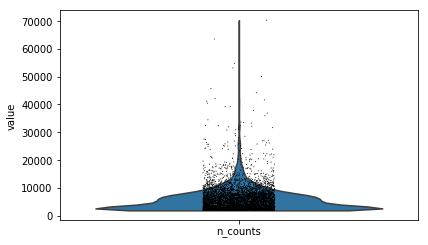
\includegraphics[width=0.22\textwidth]{GSM3308814-n-counts-violin.png}} 
    \subfigure{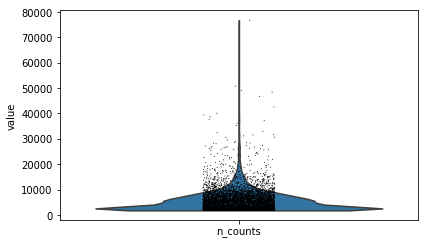
\includegraphics[width=0.22\textwidth]{GSM3308815-n-counts-violin.png}} 
    \subfigure{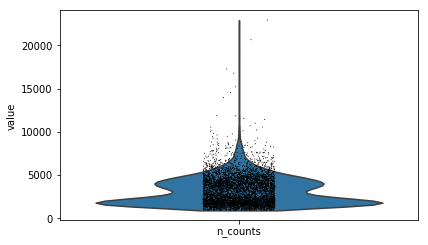
\includegraphics[width=0.22\textwidth]{GSM3316206-n-counts-violin.png}}
    \subfigure{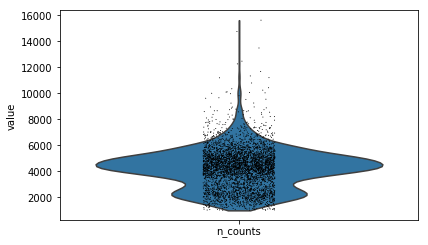
\includegraphics[width=0.22\textwidth]{GSM3316207-n-counts-violin.png}}
    \caption{ Violinski grafici količine izmerenih molekula iRNK za (a) GSM3308814 (b) GSM3308815 (c) GSM3316206 (d) GSM3316207. Na y osi na prvoj slici predstavljen je broj očitanih molekula iRNK dok x osa služi za vizuelizaciju gustine raspodele broja molekula iRNK. Crne tačke predstavljaju prave podatke i vidi se da im je najveća koncentracija tamo gde je grafik najdeblji odnosno gde je verovatnoća najveća. }
    \label{fig:n_counts_violin}
\end{figure}

Primećujemo da se najveći broj ćelija u prvoj grupi (GSM3308814 i GSM3308815) nalazi u opsegu od 0 do 10000 očitanih jedinica iRNK ali da očitane vrednosti idu čak i do 70000. Ne čudi što su rezultati ove dve datoteke gotovo identični jer je GSM3308815 samo kopiran i koristi se za verifikaciju samog procesa uzorkovanja (vidi kolonu 'DESCRIPTION' u datoteci sa metapodacima). U drugoj grupi je situacija drugačija: raspodela vrednosti ima malo nepravilniji oblik i manji opseg a uzorci su međusobno manje slični.

Kada se posmatraju violinski grafici procenta mitohondrijske RNK, primećuju se veliki procenti u prvoj grupi (raspodela je dosta široka u predelu od oko 40\%, što je mnogo više od preporučenih 20\%-25\%\cite{sstutorial}) ali još uvek neće biti izvedeni zaključci o kvalitetu uzorka zbog potencijalnih problema koji se mogu javiti i spomenuti su ranije u tekstu. Razlika između uzoraka možda potiče od različitih stupnjeva u razvoju ćelija između dva merenja. Takođe je moguće da se razlika javlja usled samog procesa merenja. 

\begin{figure}[!h]
    \centering
    \subfigure{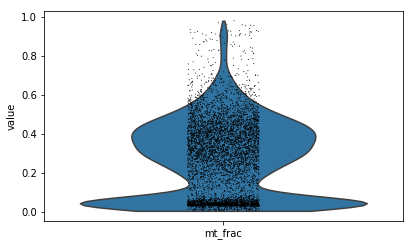
\includegraphics[width=0.2\textwidth]{GSM3308814-mt-frac-violin.png}} 
    \subfigure{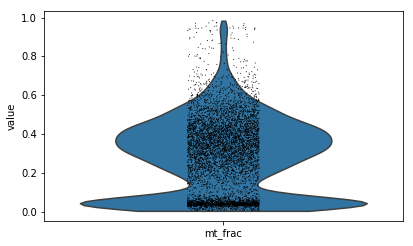
\includegraphics[width=0.2\textwidth]{GSM3308815-mt-frac-violin.png}} 
    \subfigure{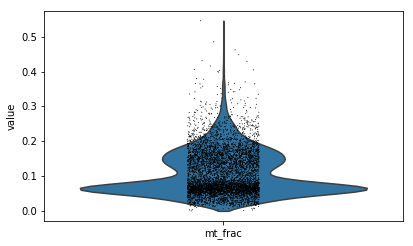
\includegraphics[width=0.2\textwidth]{GSM3316206-mt-frac-violin.png}}
    \subfigure{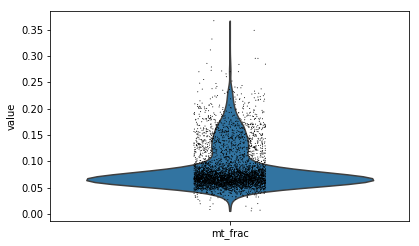
\includegraphics[width=0.2\textwidth]{GSM3316207-mt-frac-violin.png}}
    \caption{ Violinski grafici broja izraženih gena za (a) GSM3308814 (b) GSM3308815 (c) GSM3316206 (d) GSM3316207}
    \label{fig:n_counts_violin}
\end{figure}

Druga grupa uzoraka ima znatno slabije izraženu mitohondrijsku RNK koja se kreće u preporučenim okvirima (najveći deo ćelija ima manje od 20\% mitohondrijske RNK). Iako bi se samo na osnovu ovih zapažanja u vezi mtRNK moglo zaključiti da prva grupa uzoraka nema dovoljno dobar kvalitet, ovi podaci će biti korišćeni i u ostatku rada. Na slici \ref{fig:odnos} je podrobnije ispitan udeo mitohondrijske RNK u prvoj grupi kako bi se podaci dodatno modifikovali.

\begin{figure}[!h]
    \centering
    \subfigure{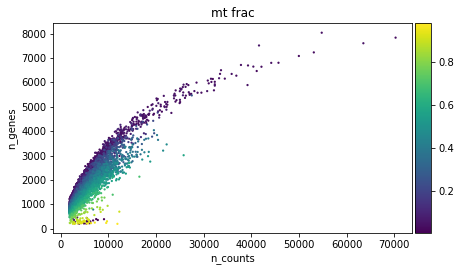
\includegraphics[width=0.45\textwidth]{GSM3308814-genes-counts.png}} 
    \subfigure{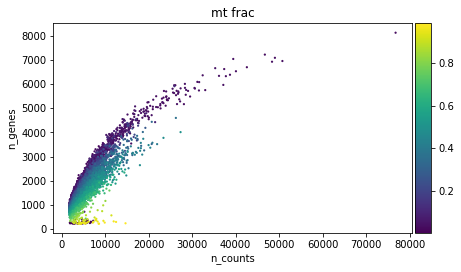
\includegraphics[width=0.45\textwidth]{GSM3308815-genes-counts.png}} 
    \caption{ Odnos između broja izraženih gena i broja očitanih molekula iRNK. Procenat mitohondrijske RNK predstavljen je uz pomoć boje (a) GSM3308814 (b) GSM3308815 }
    \label{fig:odnos}
\end{figure}

Jasno se uočava oblast tačaka sa malim brojem izraženih gena i malom količinom iRNK, a velikom koncentracijom mtRNK u donjem levom uglu na oba grafika (prikazano žutom bojom). Dobra stvar je što su nepoželjne tačke u nekoj meri linearno odvojive od glavnice podataka. Da bi se donela odluka o granicama odsecanja ovih tačaka, vršena je dodatna analiza raspodele ovih tačaka (slika \ref{fig:n_counts_GSM3308814_hist_qc}):

\begin{figure}[!h]
    \centering
    \subfigure{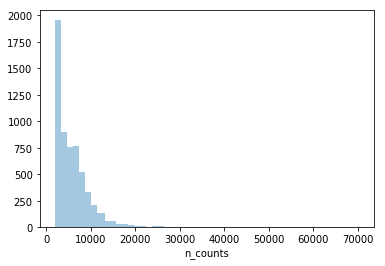
\includegraphics[width=0.45\textwidth, height=75]{GSM3308814-counts-hist.png}}
    \subfigure{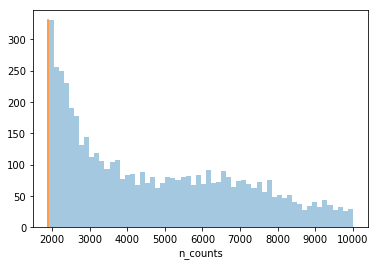
\includegraphics[width=0.45\textwidth, height=75]{GSM3308814-counts-hist-low-end.png}} 
    \subfigure{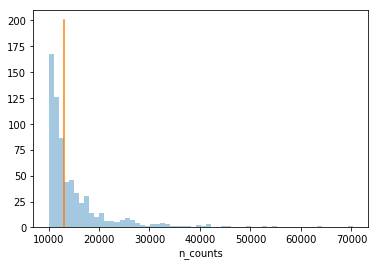
\includegraphics[width=0.45\textwidth, height=75]{GSM3308814-counts-hist-high-end.png}}
    \subfigure{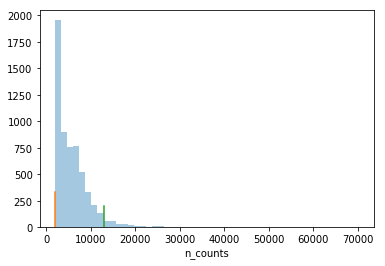
\includegraphics[width=0.45\textwidth, height=75]{GSM3308814-counts-hist-filtered.png}}
    \caption{ Raspodele broja izmerenih molekula iRNK za GSM3308814: x osa predstavlja broj izmerenih molekula iRNK, a y osa predstavlja broj ćelija (a) vidi se da najveći broj ćelija ima mali broj očitavanja (b) Uveličan deo grafika u opsegu od 0 do 10000 ; odabrana je donja granica za n\_counts 1900 (c) Uveličan deo grafika u opsegu od 10000 do 70000 ; odabrana je gornja granica za n\_counts 13000 (d) n\_counts sa gornjom i donjom granicom. Vidi se sličnost između (a) na slici \ref{fig:n_counts_violin} i (a) na ovoj slici: prva slika je dobijena tako što se histogram sa ove slike zarotirao za 90 stepeni, duplirao kao u ogledalu i "uglačao". }
    \label{fig:n_counts_GSM3308814_hist_qc}
\end{figure}

%\newpage

Nakon filtriranja podataka korišćenjem pomenutih granica, broj ćelija sa velikim procentom mtRNK je smanjen (slika \ref{fig:mt_frac_GSM14_after_filtering}). 

\begin{figure}[!ht]
    \centering
    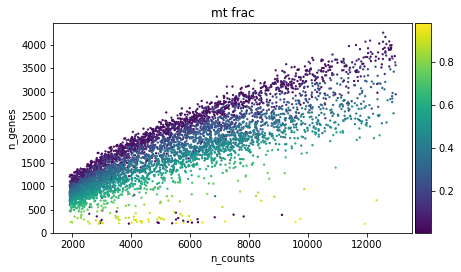
\includegraphics[width=0.45\textwidth]{GSM3308814-genes-counts-filtered.png}
    \caption{ Značajno smanjen broj ćelija sa visokim udelom mtRNK }
    \label{fig:mt_frac_GSM14_after_filtering}
\end{figure}

Na slici \ref{fig:n_genes_GSM3308814_hist_qc} su prikazani historgami broja izraženih gena u ćelijama:

\begin{figure}[!h]
    \centering
    \subfigure{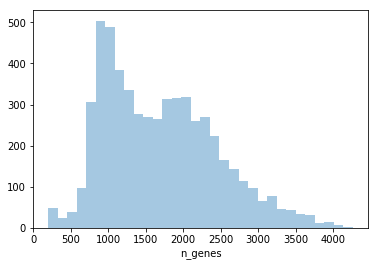
\includegraphics[width=0.45\textwidth]{GSM3308814-genes-hist.png}}
    \subfigure{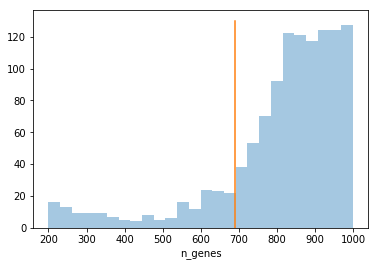
\includegraphics[width=0.45\textwidth]{GSM3308814-genes-hist-low-end.png}} 
    \subfigure{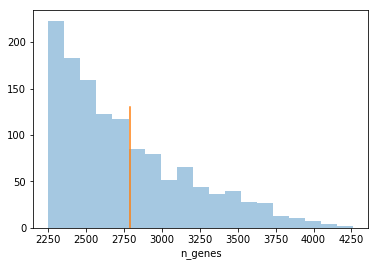
\includegraphics[width=0.45\textwidth]{GSM3308814-genes-hist-high-end.png}}
    \subfigure{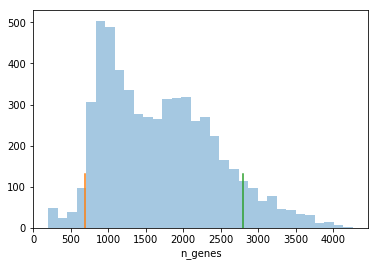
\includegraphics[width=0.45\textwidth]{GSM3308814-genes-hist-filtered.png}}
    \caption{ Raspodele broja izraženih gena za GSM3308814: na x osi je broj različitih gena izraženih po ćeliji, a na y osi je broj ćelija (a) vide se dve oblasti sa većom koncentracijom izraženih gena, oko 1000 i 2000 (b) Uveličan deo grafika u opsegu od 0 do 1000 ; odabrana je donja granica za n\_genes 690 (c) Uveličan deo grafika u opsegu od 2250 do 4250 ; odabrana je gornja granica za n\_genes 2790 (d) n\_genes sa gornjom i donjom granicom }
    \label{fig:n_genes_GSM3308814_hist_qc}
\end{figure}

Posle filtriranja dobijeni su sledeći rezultati (slika \ref{fig:n_counts_after_filtering_genes}):  

\begin{figure}[!h]
    \centering
    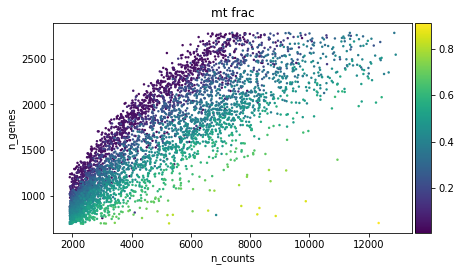
\includegraphics[width=0.45\textwidth]{GSM3308814-genes-counts-filtered2.png}
    \caption{ Broj ćelija sa visokim procentom mtRNK je dodatno smanjen }
    \label{fig:n_counts_after_filtering_genes}
\end{figure}

\newpage

Podaci iz uzorka GSM3308815 analizirani su i obrađeni analogno.

Na slici (\ref{fig:genes_counts_group_2}) za uzorke druge grupe se vidi da ne postoji neka ravan odsecanja koja bi mogla da razdvoji podatke sa velikim i malim procentima mtRNK. Takođe, najveće vrednosti za ovu vrstu RNK su oko 50\% za GSM3316206 i 35\% za GSM3316207 (vidi sliku \ref{fig:genes_counts_group_2}). Iz ovih razloga, izbačene su ćelije sa više od 20\% nakon čega se broj ćelija smanjio sa 6053 na 5513 u GSM3316206 i sa 4222 na 4120 u GSM3316207 (slika \ref{fig:genes_counts_filtered_group_2}).

\begin{figure}[!h]
    \centering
    \subfigure{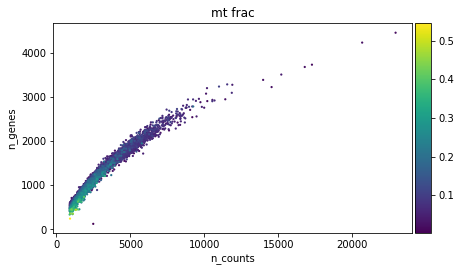
\includegraphics[width=0.45\textwidth]{GSM3316206-genes-counts.png}}
    \subfigure{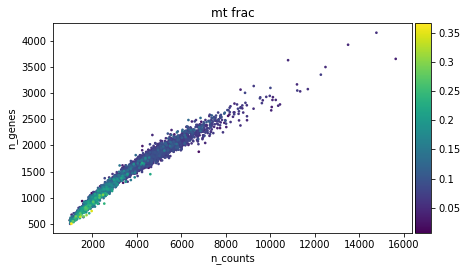
\includegraphics[width=0.45\textwidth]{GSM3316207-genes-counts.png}} 
    \caption{ (a) GSM3316206 (b) GSM3316207 }
    \label{fig:genes_counts_group_2}
\end{figure}

\begin{figure}[!h]
    \centering
    \subfigure{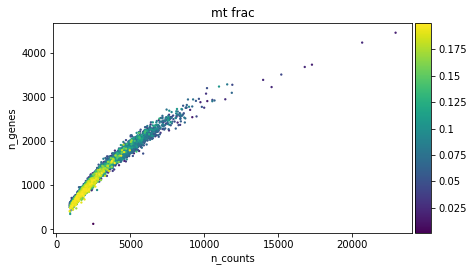
\includegraphics[width=0.45\textwidth]{GSM3316206-genes-counts-filtered.png}}
    \subfigure{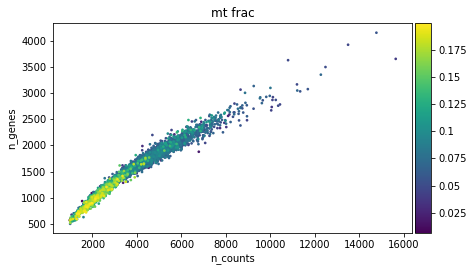
\includegraphics[width=0.45\textwidth]{GSM3316207-genes-counts-filtered.png}} 
    \caption{ (a) GSM3316206 (b) GSM3316207 }
    \label{fig:genes_counts_filtered_group_2}
\end{figure}

\subsubsection{Normalizacija}

Pošto sigurno nisu svi molekuli iRNK pokupljeni prilikom uzorkovanja, može se desiti da broj molekula varira između ćelija što može biti posledica samog uzorkovanja. Pošto se ne može pretpostaviti da je broj molekula iRNK u svim ćelijama isti, cilj je normalizacijom modifikovati vrednosti tako da dovoljno dobro procenjuju stvaran broj molekula u ćeliji. Ne procenjuje se sam broj molekula, već faktori u okviru svake ćelije koji bi trebalo da budu proporcionalni broju molekula ćelija - \textbf{faktori velilčine}. Normalizacija se vrši tako što se izmerene vrednosti dele odgovarajućim faktorima. U okviru paketa scanpy, vrši se CPM (counts per million) normalizacija: $CPM = \frac{\frac{r_i}{R}}{10^6}$, gde je $R$ broj registrovanih molekula u celom uzorku, a $r_i$ su brojevi molekula za svaki atribut, rezultati se skaliraju sa milion zarad bolje čitljivosti. Nakon toga se podaci logaritmuju. Normalizacija je bitan korak u obradi podataka\cite{luecken2019current, long2019cluster} i zato je primenjena u ovom radu.

\subsubsection{Vizualizacija}

Podaci sa kojima se rade imaju ogromne dimenzije i nije moguće vizuelno ih predstaviti. Sa druge strane, veliki broj tih dimenzija nema nikakvu ulogu u istraživanju latentnih informacija. Stoga je neophodno smanjenje broja dimenzija podataka. 

Tehnike za smanjenje dimenzionalnosti podataka korišćene u ovom radu su \textbf{PCA}, \textbf{tSNE} i \textbf{UMAP}.

\paragraph{PCA} je tehnika smanjenja dimenzija podataka koja akcenat stavlja na varijabilnost, odnosno nastoji da predstavi samo one dimenzije koje pokrivaju najveću varijabilnost u okviru podataka. Početan visokodimenzionalan skup se linearnim transformacijama dovodi u skup sa manjim brojem dimenzija, odnosno glavnih komponenti koje su međusobno linearno nezavisne.

\paragraph{tSNE} Za razliku od PCA, tSNE ne koristi linearnu transformaciju već se oslanja na lokalne odnose između podataka i stoga je sposobna da prepozna i nelinearne strukture. Uz pomoć normalne raspodele, pravi se raspodela u visokodimenzionom prostoru i nakon toga se uz pomoć studentove t-raspodele rekonstruišu ti odnosi u nižim dimenzijama. Više detalja u \cite{maaten2008visualizing, wattenberg2016how}

\paragraph{UMAP} predstavlja poboljšanje tSNE algoritma, odnosno brže se izvršava, bolje čuva globalnu strukturu podataka i takođe ima svrhu i van same vizualizacije pa se koristi i kao generalna tehnika smanjenja dimenzionalnosti podataka. U suštini, sastoji se iz dva koraka: 1) konstrukcija grafa povezanosti u visokodimenzionom prostoru i 2) optimizacija tog grafa koja traži najsličniju reprezentaciju u nižim dimenzijama. Više detalja može se naći u \cite{mcinnes2018umap, umapexplain}

Bitno je napomenuti nekoliko stvari u vezi tSNE i UMAP projekcija podataka. Naime, veličina klastera (površina koju klaster zauzima na slici, a ne broj samih tačaka u tim klasterima) na ovim projekcijama ne mora da znači gotovo ništa. Ovo je posledica toga što i tSNE i UMAP koriste lokalne udaljenosti za projektovanje u nižu dimenziju. tSNE algoritam će zato "širiti" guste klastere, a "sabijati" rasprsnute i na taj način će ih izjednačiti. Stoga, nije moguće uzimati u obzir relativne veličine klastera i iz njih izvlačiti ikakve zaključke. Još jedna stvar oko koje treba biti oprezan prilikom tumačenja ovih projekcija je da distance između dobro razdvojenih klastera često nemaju značenje što je još jedna posledica korišćenja lokalnih udaljenosti u algoritmu. Pošto su oba algoritma stohastička, odnosno mogu dati različite rezultate svaki put kada se izvrše, nekada je potrebno više puta ih pokrenuti zbog realnije slike o podacima.

Iako su ove dve tehnike dobre za prikaz visokodimenzionog prostora u manje dimenzija i dobro oslikavaju lokalnu povezanost tačaka u okviru istih klastera, treba biti svestan i navedenih zamki prilikom tumačenja grafika dobijenih ovim tehnikama. 

\begin{figure}[!h]
    \centering
    \subfigure{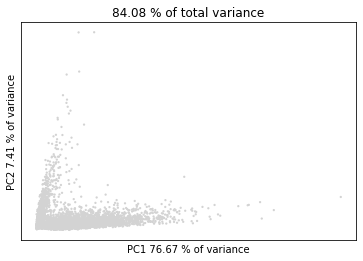
\includegraphics[width=0.25\textwidth, height=75]{pca-14.png}}
    \subfigure{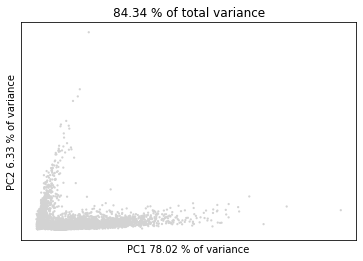
\includegraphics[width=0.25\textwidth, height=75]{pca-15.png}} 
    \caption{ Dimenziono redukovani podaci na dve glavne komponente sa najvećom varijansom korišćenjem PCA dekompozicije: ose na ovom grafiku predstavljaju dva pravca u kojima je varijansa najveća. Ose su zapravo linearne kombinacije visokodimenzionog prostora. Ispod svake slike je oznacen procenat varijanse koji pokriva odredjena glavna komponenta, i zato su razlike u pravcu x ose bitnije od razlika u pravcu y ose. (a) GSM3308814: jasno se uočava da su podaci rasporedjeni u dva pravca (prve dve glavne komponente pokrivaju oko 84\% varijanse u obe datoteke) (b) GSM3308815: podaci deluju gotovo identicno prvoj datoteci. Ova zapazanja nam govore da ce u daljoj analizi biti moguce smanjiti dimenzionalnost podataka bez velikih gubitaka informacija. }
    \label{fig:pca_HVG_group_1}
\end{figure}

\begin{figure}[!h]
    \centering
    \subfigure{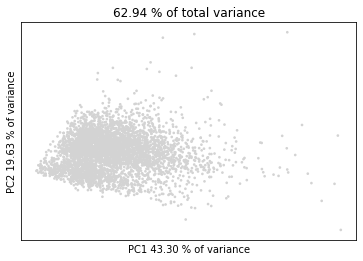
\includegraphics[width=0.25\textwidth, height=75]{pca-206.png}}
    \subfigure{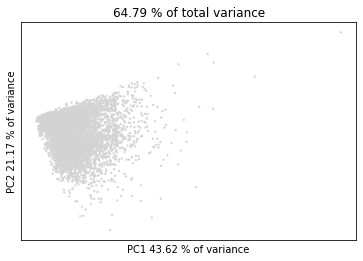
\includegraphics[width=0.25\textwidth, height=75]{pca-207.png}} 
    \caption{ (a) GSM3316206: situacija je malo drugacija sto je i ocekivano s obzirom da prve dve komponente pokrivaju manji procenat varijanse. (b) GSM3316207: sve tačke su veoma slične. U ovom slucaju, potrebno nam je vise glavnih komponenti u odnosu na prvu grupu za istu pokrivenost varijanse. }
    \label{fig:pca_HVG_group_2}
\end{figure}

PCA nam očigledno ne pruža dovoljno informacija za zaključivanje o pripadnosti nekom klasteru, ali nam može koristiti kao smernica za izbor broja glavnih komponenti. Na osnovu grafika pokrivenosti varijanse u odnosu na broj glavnih komponenti, biće izabran broj komponenti za konstrukciju grafa suseda (slika \ref{fig:pca_HVG_group_1}). 

\begin{figure}[!h]
    \centering
    \subfigure{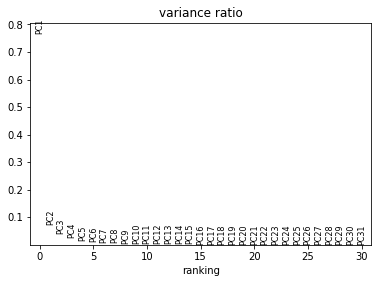
\includegraphics[width=0.2\textwidth]{14-variance-ratio.png}}
    \subfigure{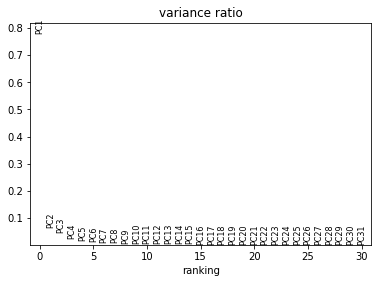
\includegraphics[width=0.2\textwidth]{15-variance-ratio.png}} 
    \subfigure{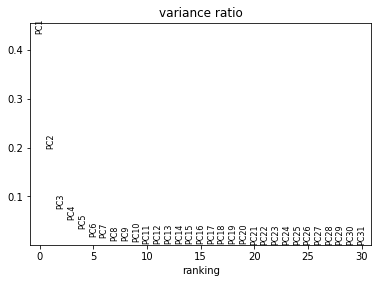
\includegraphics[width=0.2\textwidth]{206-variance-ratio.png}}
    \subfigure{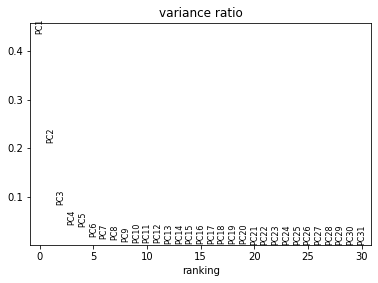
\includegraphics[width=0.2\textwidth]{207-variance-ratio.png}} 
    \caption{ Prikaz odnosa broja komponenti i procenta pokrivenosti varijanse. Često se ovaj prikaz koristi za odabir broja glavnih komponenti, ali ovde će biti korišćen drugačiji pristup. Naime, biće izabran dovoljan broj glavnih komponenti da se pokrije određen procenat varijanse. }
    \label{fig:variance_ratios}
\end{figure}

Za UMAP i tSNE vizualizacije potrebna je konstrukcija grafa susedstva za date podatke. Grafovi su konstruisani metodom \lstinline{sc.pp.neighbors} paketa \lstinline{scanpy}. Za svaki skup podataka korisceno je po dve razlicite metrike: euklidsko i kosinusno. Broj glavnih komponenti odabran je tako da je pokriveno barem 90\% varijanse u svakom skupu (vidi sliku \ref{fig:variance_ratios}).

\begin{figure}[!h]
    \centering
    \subfigure{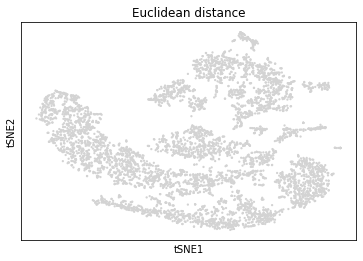
\includegraphics[width=0.3\textwidth, height=75]{euclidean-14-tsne.png}}
    \subfigure{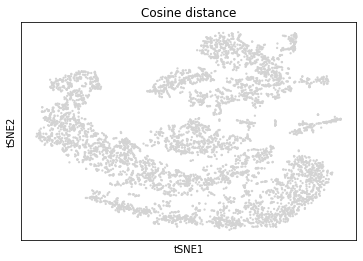
\includegraphics[width=0.3\textwidth, height=75]{cosine-14-tsne.png}} 
    \caption{ GSM3308814 (a) tSNE vizualizacija koriscenjem euklidskih rastojanja: sa slike se moze zakljuciti da postoji preko 5 klastera, ali treba uzeti u obzir i navedene mere opreza, odnosno suzdrzati se od tumacenja razdvojenosti i oblika klastera. Ova tehnika nam pruza preliminarni uvid u podatke i imace vise smisla kada bude primenjeno klasterovanje.  (b) kosinusna rastojanja: I ovde se vidi preko pet klastera malo drugacijeg oblika. Ono sto se moze videti sa slike je reprezentacija topologije podataka u dvodimenzionom prostoru. }
    \label{fig:visualize_14_tsne}
\end{figure}

\begin{figure}[!h]
    \centering
    \subfigure{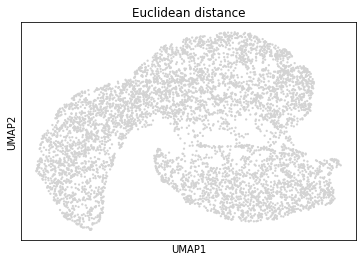
\includegraphics[width=0.3\textwidth, height=75]{euclidean-14-umap.png}}
    \subfigure{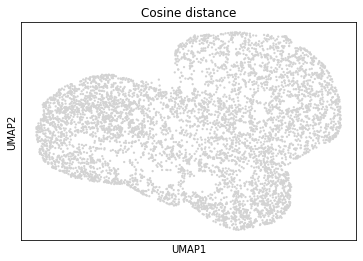
\includegraphics[width=0.3\textwidth, height=75]{cosine-14-umap.png}} 
    \caption{ GSM3308814 (a) UMAP vizualizacija koriscenjem euklidskih rastojanja: jasno je razdvojeno dva klastera, ali treba uzeti u obzir i navedene mere opreza, odnosno suzdrzati se od tumacenja razdvojenosti grafova. Ova tehnika nam pruza preliminarni uvid u podatke i imace vise smisla kada bude primenjeno klasterovanje.  (b) kosinusna rastojanja: podaci deluju malo slicnije i sa ove slike se ne moze puno zakljuciti, bice lakse tumaciti rezultate nakon klasterovanja. Ono sto se moze videti sa slike je reprezentacija topologije podataka u dvodimenzionom prostoru. Takodje se moze videti da su podaci manje razdvojeni u odnosu na tSNE vizualizaciju, ali i tu treba biti oprezan jer je za UMAP poznato da bolje cuva globalnu topologiju. }
    \label{fig:visualize_14_umap}
\end{figure}

Primećuje se da tSNE grafici uglavnom daju veliki broj klastera sa delimično nejasnim granicama, dok se UMAP vizualizacije ponašaju relativno bolje. UMAP algoritam se brže izvršava i bolje oslikava topologiju podataka. Vizualizacije neklasterovanih podataka su u dodatku\ref{}. U nastavku ce biti koriscena UMAP vizualizacija, a tSNE vizualizacije mogu se dobiti pokretanjem metoda iz skripta clustering.

\section{Klasterovanje}

Za klasterovanje će biti korišćeni algoritmi louvain i leiden implementirani u okviru scanpy paketa. Takođe će biti izvršeni algoritmi za klasterovanje prisutni u scikit-learn paketu. Kod koji je korišćen za dobijanje navedenih rezultata nalazi se u skripti cluster. Rezultati klasterovanja sa ocenama kvaliteta i ćelijama koje pripadaju svakom klasteru dati su u okviru foldera clustering\_results.

\subsubsection{Louvain i Leiden}

\paragraph{Louvain\cite{blondel2008fast,traag2019louvain}} je algoritam hijerarhijskog klasterovanja koji otkriva klastere u mrežama tako što maksimizuje nivo modularnosti svakog klastera. To znači da se procenjuje koliko su jako povezani čvorovi nekog klastera u odnosu na to koliko bi bili povezani u nasumičnoj mreži. Rekurzivno se spajaju klasteri i primenjuje se maksimizacija modularnosti na spojenim klasterima.
Matematička formulacija modularnosti:
$$
H = \frac{1}{2m}\sum_{c} (e_c - \gamma\frac{K_c^2}{2m})
$$
Gde je $K_c$ suma stepeni čvorova u klasteru $c$, $m$ je ukupan broj grana u mreži, $e_c$ je broj grana u klasteru $c$ i $\gamma$ je rezolucija. Veća rezolucija dovodi do većeg broja klastera a manja do manjeg.


\paragraph{Leiden\cite{traag2019louvain}} algoritam predstavlja poboljšanje louvain algoritma u kome se može desiti da neki čvor koji je imao ulogu spone između klastera uđe u sastav nekog novog klastera i na taj način napravi nepovezane klastere. Ovo se rešava uvođenjem dodatnog međukoraka prečišćavanja klastera. U tom koraku se čvorovi ne pridružuju nužno onom klasteru za koji je modularnost najveća već se nasumično bira neki od klastera za koji se povećava ciljna funkcija.


U nastavku ce biti prikazani najbolji (po koeficijentu senke) rezultati za ova dva algoritma klasterovanja po datotekama. Algoritmi su pokrenuti za interval rezolucija od 1.0 do 0.15. Ovaj parametar odredjuje koliko blizu tacke trebaju biti medjusobno kako bi se smestile u isti klaster. Vece vrednosti daju vise klastera, odnosno lokalna slicnost je naglasenija, dok manje vrednosti ovog parametra daju manji broj klastera sa vise tacaka.

U sledecoj tabeli dati su najbolji rezultati klasterovanja u odnosu na koeficijent senke i Davies-Bouldin indeks.

\begin{table}[!h]
\resizebox{\textwidth}{!}{%
\begin{tabular}{lllllllll}
\cline{2-9}
\multicolumn{1}{l|}{} & \multicolumn{2}{l|}{\textbf{GSM3308814}} & \multicolumn{2}{l|}{\textbf{GSM3308815}} & \multicolumn{2}{l|}{\textbf{GSM3316206}} & \multicolumn{2}{l|}{\textbf{GSM3316206}} \\ \cline{2-9} 
\multicolumn{1}{l|}{} & \multicolumn{2}{l}{Distance used} & \multicolumn{2}{l}{Distance used} & \multicolumn{2}{l}{Distance used} & \multicolumn{2}{l}{Distance used} \\ \cline{5-5}
\multicolumn{1}{l|}{\multirow{-3}{*}{}} & Euclidean & Cosine & \multicolumn{1}{l|}{Euclidean} & \multicolumn{1}{l|}{\cellcolor[HTML]{67FD9A}Cosine} & Euclidean & Cosine & Euclidean & Cosine \\ \cline{1-1} \cline{5-5}
\multicolumn{1}{|l|}{\cellcolor[HTML]{FD6864}Silhouette} & 0.3446 & 0.3933 & \multicolumn{1}{l|}{0.3723} & \multicolumn{1}{l|}{\cellcolor[HTML]{FD6864}{\color[HTML]{000000} 0.4737}} & 0.3853 & 0.3109 & 0.4015 & 0.3695 \\ \cline{1-1} \cline{5-5}
\multicolumn{1}{|l|}{\cellcolor[HTML]{FE996B}Calinski-Harabasz} & 7202.4210 & 7892.7844 & \multicolumn{1}{l|}{7390.1634} & \multicolumn{1}{l|}{\cellcolor[HTML]{FE996B}9046.2576} & 3368.4585 & 3186.1564 & 5616.0195 & 2916.7540 \\ \cline{1-1} \cline{5-5}
\multicolumn{1}{|l|}{\cellcolor[HTML]{FFFE65}Davies-Bouldin} & 0.9388 & 0.7874 & \multicolumn{1}{l|}{\cellcolor[HTML]{FFFE65}0.6779} & \multicolumn{1}{l|}{\cellcolor[HTML]{67FD9A}0.7431} & 0.8893 & 0.8316 & 0.7750 & 1.0421 \\ \cline{1-1} \cline{5-5}
\multicolumn{1}{|l|}{Resolution} & 0.3 & 0.15 & \multicolumn{1}{l|}{0.15} & \multicolumn{1}{l|}{\cellcolor[HTML]{67FD9A}0.15} & 0.15 & 0.5 & 0.3 & 0.15 \\ \cline{1-1} \cline{5-5}
\multicolumn{1}{|l|}{Clusters found} & 8 & 5 & \multicolumn{1}{l|}{6} & \multicolumn{1}{l|}{\cellcolor[HTML]{67FD9A}4} & 3 & 7 & 5 & 3 \\ \cline{1-1} \cline{5-5}
\end{tabular}%
}
\caption{Rezultati klasterovanja koriscenjem louvan algoritma: iz tabele se vidi da je najbolji rezultat (2 od 3 najbolje ocene) klasterovanje datoteke GSM3308815 za rezoluciju 0.15. Ovaj rezultat nije toliko ocigledan na slici\ref{fig:best_louvain} sto je i ocekivano s obzirom da su brojcane vrednosti ocena veoma bliske. Generalno se vidi da se za prvu grupu (GSM3308814 i GSM3308815) kosinusna rastojanja bolje ponasaju od euklidskih dok je za druge dve datoteke situacija suprotna. Iako postoje razlike izmedju izbora metrika rastojanja, ne deluje da su toliko znacajne.  } \label{tab:louvain-results}
\end{table}

\begin{figure}[!h]
    \centering
    \subfigure{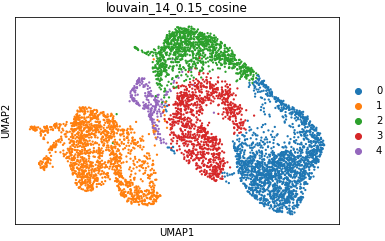
\includegraphics[width=0.22\textwidth]{louvain-14-best.png}} 
    \subfigure{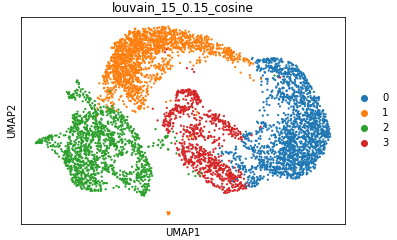
\includegraphics[width=0.22\textwidth]{louvain-leiden-15-best.png}} 
    \subfigure{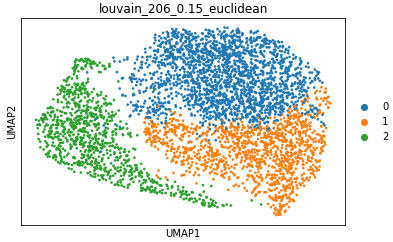
\includegraphics[width=0.22\textwidth]{louvain-206-best.png}}
    \subfigure{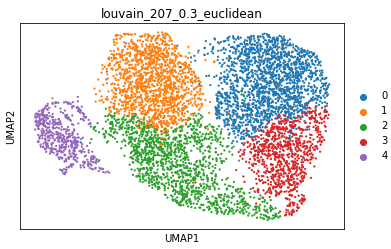
\includegraphics[width=0.22\textwidth]{louvain-207-best.png}}
    \caption{ UMAP reprezentacija rezultata najboljih klasterovanja za algoritam Louvain po datotekama. U prvoj grupi (a) i (b) deluje da je algoritam odradio dosta dobar posao i da je na logican nacin razdvojio kalstere. Kao sto je vec spomenuto, velicina ovih klastera ne mora da ima bilo kakvo znacenje, bitno je da su tacke u okviru klastera medjusobno slicne. Takodje udaljenost klastera nema neku posebnu vaznost. Sa slika se moze videti topoloska organizacija podataka projektovana na 2 dimenzije. Na slici pod (a) vidimo da su klasteri "prosarani" i tackama koje mozda logicno ne bi trebalo smestiti u njih, sto je potvrdjeno i koeficijentom senke koji je relativno mali. Na slici (b) se takodje vide neke tacke koje odstupaju. Slicna situacija je i sa slikama (c) i (d) s tim sto deluje da je algoritam pronasao vise klastera nego sto bi se golim okom procenilo, odnosno na slici (c) bi se klasteri 0 i 1 mogli spojiti u jedan veci na osnovu slike, a na slici (d) bi se klasteri 1 i 2 mogli spojiti u jedan, a klasteri 0 i 3 spojiti u drugi klaster na taj nacin formirajuci samo tri klastera. Povecan prostor pretrage za parametar rezolucije bi mozda proizveo bolje rezultate, ali u eksperimentima nije doslo do poboljsanja i ovo su najbolji rezultati nakon vise pokusaja. U nastavku ce takodje biti dati najbolji dobijeni rezultati. }
    \label{fig:best_louvain}
\end{figure}

\begin{table}[!h]
\resizebox{\textwidth}{!}{%
\begin{tabular}{lllllllll}
\cline{2-9}
\multicolumn{1}{l|}{} & \multicolumn{2}{l|}{\textbf{GSM3308814}} & \multicolumn{2}{l|}{\textbf{GSM3308815}} & \multicolumn{2}{l|}{\textbf{GSM3316206}} & \multicolumn{2}{l|}{\textbf{GSM3316206}} \\ \cline{2-9} 
\multicolumn{1}{l|}{} & \multicolumn{2}{l}{Distance used} & \multicolumn{2}{l}{Distance used} & \multicolumn{2}{l}{Distance used} & \multicolumn{2}{l}{Distance used} \\ \cline{5-5}
\multicolumn{1}{l|}{\multirow{-3}{*}{}} & Euclidean & Cosine & \multicolumn{1}{l|}{Euclidean} & \multicolumn{1}{l|}{Cosine} & Euclidean & Cosine & Euclidean & Cosine \\ \cline{1-1} \cline{5-5}
\multicolumn{1}{|l|}{\cellcolor[HTML]{FD6864}Silhouette} & 0.3561 & \cellcolor[HTML]{FD6864}0.4199 & \multicolumn{1}{l|}{0.4045} & \multicolumn{1}{l|}{0.3968} & 0.3363 & 0.3421 & 0.4054 & 0.3830 \\ \cline{1-1} \cline{5-5}
\multicolumn{1}{|l|}{\cellcolor[HTML]{FE996B}Calinski-Harabasz} & 6646.1356 & 7531.1001 & \multicolumn{1}{l|}{\cellcolor[HTML]{FE996B}7754.5354} & \multicolumn{1}{l|}{6914.3054} & 3271.5613 & 3092.7325 & 4770.8381 & 3512.9175 \\ \cline{1-1} \cline{5-5}
\multicolumn{1}{|l|}{\cellcolor[HTML]{FFFE65}Davies-Bouldin} & 0.8271 & 1.3735 & \multicolumn{1}{l|}{\cellcolor[HTML]{FCFF2F}0.7408} & \multicolumn{1}{l|}{0.9940} & 0.9888 & 0.8927 & 0.7530 & 0.8721 \\ \cline{1-1} \cline{5-5}
\multicolumn{1}{|l|}{Resolution} & 0.15 & 0.15 & \multicolumn{1}{l|}{0.15} & \multicolumn{1}{l|}{0.3} & 0.5 & 0.3 & 0.15 & 0.15 \\ \cline{1-1} \cline{5-5}
\multicolumn{1}{|l|}{Clusters found} & 5 & \cellcolor[HTML]{D6F2D6}5 & \multicolumn{1}{l|}{\cellcolor[HTML]{D6F2D6}6} & \multicolumn{1}{l|}{8} & 7 & 5 & 4 & 4 \\ \cline{1-1} \cline{5-5}
\end{tabular}%
}
\caption{Rezultati klasterovanja koriscenjem leiden algoritma: iz tabele se vidi da je najbolji rezultat (2 od 3 najbolje ocene) klasterovanje datoteke GSM3308815 za rezoluciju 0.15 i euklidsko rastojanje. S druge strane, klasterovanje za datoteku GSM3308814 i kosinusno rastojanje daje bolju ocenu senke, tako da nije najjasnije koji klaster je bolji. Zanimljivo je da ovde nema pravilnosti vezanih za izbor ocene rastojanja i kvaliteta klasterovanja prvu datoteku je bolje kosinusno, za drugu euklidsko, za trecu kosinusno i za cetvrtu euklidsko. Ni sada rezultati nisu toliko uocljivi na slici \ref{fig:leiden-best} } \label{tab:leiden-results}
\end{table}

\begin{figure}[!h]
    \centering
    \subfigure{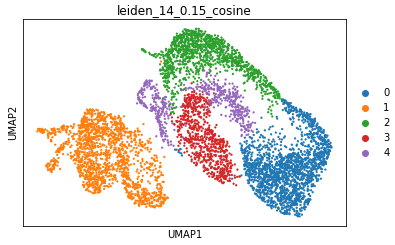
\includegraphics[width=0.22\textwidth]{leiden-14-best.png}} 
    \subfigure{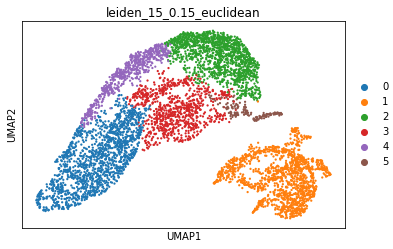
\includegraphics[width=0.22\textwidth]{leiden-15-best.png}} 
    \subfigure{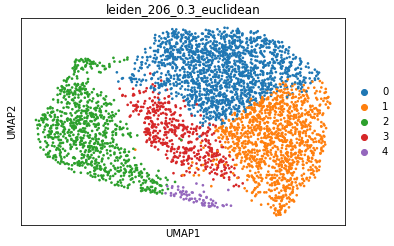
\includegraphics[width=0.22\textwidth]{leiden-206-best.png}}
    \subfigure{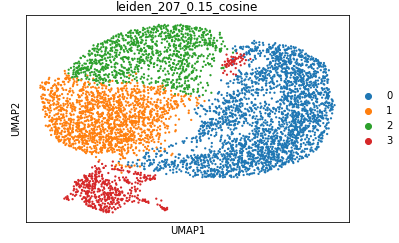
\includegraphics[width=0.22\textwidth]{leiden-207-best.png}}
    \caption{ UMAP reprezentacija rezultata najboljih klasterovanja za algoritam leiden po datotekama: Slicna je situacija kao i kod louvain algoritma, na prvi pogled podaci deluju smisleno organizovano u klastere s tim da su na nekim mestima prosarani tackama koje mozda ne pripadaju datoj okolini. Na primer, na slici (a) se vidi da je klaster 4 dosta razvucen i da su tacke koje mu pripadaju dosta udaljene jedne od drugih. Takodje se moze primetiti mala grupa tacaka klastera 0 u donjem levom uglu klastera 3 sto je takodje zanimljivo. Na slici (b) postoji malo manje ovakvih anomalija i klasteri su generalno dobro razdvojeni i moze se reci da bi se i rucno slicno izdvojili klasteri. Na slici (d) izgleda kao da je algoritam pronasao vise klastera nego sto je ih je vizuelno, ali opet treba naglasiti da se kod tumacenja UMAP reprezentacije rastojanje izmedju klastera treba uzeti sa rezervom. Na slici (d) vidimo crvene tacke koje "upadaju" u region koji uglavnom zauzimaju plave tacke. U poredjenju sa louvain algoritmom, (a) ima bolji koeficijent senke, a gore Calinski-Harabasz i Davies-Bouldin indekse. Prilikom poredjenja slika (a) takodje se moze primetiti da se ljubicasti klasteri razlikuju, odnosno da je louvain algoritam pronasao malo logicniju podelu. Slike pod (b) i (d) se ne mogu porediti jer je za vizualizaciju koriscena drugacija metrika u ovim algoritmima, ali mozemo im uporediti ocene i zakljuciti da je leiden algoritam za euklidsko rastojanje u datotedci GSM3308815 nasao malo bolje klastere u odnosu na pokretanje louvain algoritma za iste parametre. S druge strane, koriscenje kosinusnog rastojanja dovelo je do znatno veceg kvaliteta klastera koriscenjem louvain algoritma. Uz to, louvain klasterovanje je pronaslo 4 klastera sto je blize broju od 5 ocekivanih klastera u podacima\cite{PBMC_ANN_classification}. Za klasterovanje predstavljeno slikom (d) dobijeni su slicni rezultati za euklidsko rastojanje koriscenjem oba algoritma. Leiden se pokazao malo bolje kada je koristio kosinusna rastojanja. Kada se uiporede slike za ova dva algoritma i datoteku GSM3316207 deluje da su klasteri lepse razdvojeni koriscenjem louvain algoritma i euklidskih rastojanja sto je i potvrdjeno unosima u tabeli. }
    \label{fig:best_leiden}
\end{figure}

Rezolucije klasterovanja je izabrane su eksperimentalno. Zbog nepoznatih stvarnih klasa uzoraka, kvalitet pronađenih klastera je procenjen merama koje ne zahtevaju oznake stvarnih klasa. Korišćeni su: Calinski-Harabasz\cite{calinskiharabasz} indeks, Davies-Bouldin\cite{davies1979cluster} indeks i koeficijent senke.

\subsubsection{KMeans klasterovanje}

Ideja algoritma je da pokuša da rasporedi podatke u k klastera tako da rastojanje među podacima u okviru jednog klastera bude minimalno. Od korisnika očekuje da unese željeni broj klastera. Rad algoritma je testiran na intervalu od 2 do 10 klastera. Dobro se skalira i na više dimenzije. Funkcija koja se minimizuje definisana je kao $$\sum_{i=0}^{n}\min_{\mu_j \in C}(||x_i - \mu_j||^2)$$
Gde je $\mu_i$ srednja vrednost podataka u klasteru $i$ a $x_i$ su sami podaci. Zbog formulacije ove formule, KMeans algoritam ne radi dobro za izdužene ili podatke nepravilnog oblika. Vizuelizacija najboljih rezultata (po koeficijentu senke) na slici \ref{fig:best_kmeans}.

\begin{table}[h!]
\resizebox{\textwidth}{!}{%
\begin{tabular}{|c|c|c|c|c|c|c|c|c|}
\hline
 & \multicolumn{2}{c|}{GSM3308814} & \multicolumn{2}{c|}{GSM3308815} & \multicolumn{2}{c|}{GSM3316207} & \multicolumn{2}{c|}{GSM3316207} \\ \hline
 & Euclidean & Cosine & Euclidean & Cosine & Euclidean & Cosine & Euclidean & Cosine \\ \hline
\cellcolor[HTML]{FD6864}Silhouette & \cellcolor[HTML]{34FF34}0.4059 & 0.3583 & 0.3719 & 0.3932 & 0.3020 & 0.3325 & 0.3600 & 0.3293 \\ \hline
\cellcolor[HTML]{FE996B}Calinski-Harabasz & \cellcolor[HTML]{34FF34}5390.8242 & 3518.0090 & 3283.3920 & 4471.3486 & 1824.6711 & 2308.4630 & 3969.1302 & 3338.0132 \\ \hline
\cellcolor[HTML]{FFFE65}Davies-Bouldin & \cellcolor[HTML]{34FF34}0.7037 & 0.7942 & 0.8642 & 0.7426 & 1.1715 & 1.0531 & 0.8804 & 0.9125 \\ \hline
k & \cellcolor[HTML]{34FF34}4 & 2 & 2 & 2 & 2 & 2 & 3 & 3 \\ \hline
\end{tabular}%
}
\caption{Rezultati klasterovanja algoritmom k-sredina: najbolje se pokazalo klasterovanje datoteke GSM3308814 i to sa k = 4, i uz koriscenje euklidskog rastojanja. Vrednosti ocena najboljih klastera su slicne onima dobijenim i za louvain i leiden klasterovanja. Rezultati su vizuelno predstavljeni na slici \ref{fig:best_kmeans} }
\label{tab:kmeans-results}
\end{table}

\begin{figure}[!h]
    \centering
    \subfigure{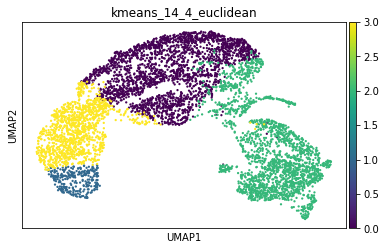
\includegraphics[width=0.22\textwidth]{kmeans-14-best.png}} 
    \subfigure{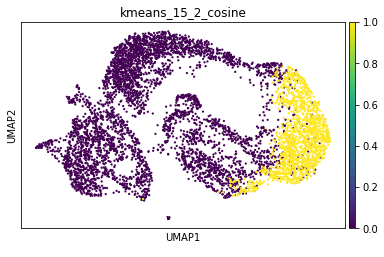
\includegraphics[width=0.22\textwidth]{kmeans-15-best.png}} 
    \subfigure{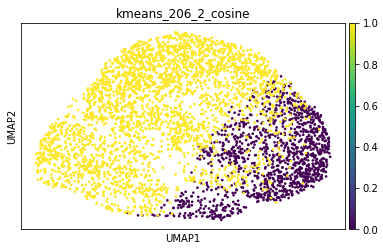
\includegraphics[width=0.22\textwidth]{kmeans-206-best.png}}
    \subfigure{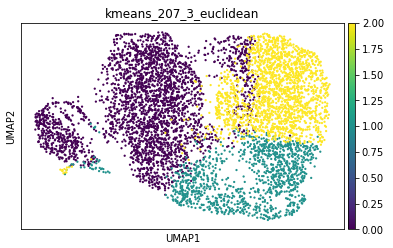
\includegraphics[width=0.22\textwidth]{kmeans-207-best.png}}
    \caption{ Vizualizacija rezultata dobijenih algoritmom k sredina: najbolje klasterovanje je dobijeno na slici (a) ali se jasno vidi nedostatak ovog algoritma jer se cini da su klasteri podeljeni gotovo linearno i uprkos solidnim ocenama iz \ref{tab:kmeans-results}, ne deluje da je podela toliko logicna. Za preostale datoteke, pogotovo na (b) i (c) se uocava isti problem i tu je razlika u odnosu na prethodne algoritme primetna i po ocenama kvaliteta. Uocljive su i tacke jednog klastera koje zalaze u druge, pogotovo na slici (d). }
    \label{fig:best_kmeans}
\end{figure}


\subsubsection{Ward klasterovanje}

Ovde će biti prikazani rezultati hijerarhijskog klasterovanja korišćenjem ward-ove veze. Opšta ideja algoritama hijerarhijskog klasterovanja je da svaki podatak u početku predstavlja jedan klaster. Iteraciju po iteraciju, klasteri se na osnovu sličnosti spajaju u veće klastere sve dok svi podaci ne upadnu u isti klaster. U okviru modula scikit-learn programskog jezika python postoji metod za ovu vrstu klasterovanja u kojoj je moguće postaviti traženi broj klastera. Kako bi se lakše poredili različiti algoritmi, i ovde je izabran interval od 2 do 10 klastera. Wardova veza minimizuje sumu kvadriranih razlika između svih klastera i zbog toga što se na taj način minimizuje varijansa, slična je KMeans algoritmu. Vizuelizacija rezultata je na slici \ref{fig:best_ward}.

\begin{table}[h!]
\resizebox{\textwidth}{!}{%
\begin{tabular}{ccccccccc}
\cline{2-9}
\multicolumn{1}{c|}{} & \multicolumn{2}{c|}{\textbf{GSM3308814}} & \multicolumn{2}{c|}{\textbf{GSM3308815}} & \multicolumn{2}{c|}{\textbf{GSM3316206}} & \multicolumn{2}{c|}{\textbf{GSM3316206}} \\ \cline{2-9} 
 & Euclidean & Cosine & Euclidean & Cosine & Euclidean & Cosine & Euclidean & Cosine \\ \cline{1-1}
\multicolumn{1}{|c|}{\cellcolor[HTML]{FD6864}Silhouette score} & \cellcolor[HTML]{FD6864}0.5193 & 0.3428 & 0.3849 & 0.4543 & 0.3265 & 0.2970 & 0.3673 & 0.3403 \\ \cline{1-1}
\multicolumn{1}{|c|}{\cellcolor[HTML]{FE996B}Calinski-Harabasz score} & \cellcolor[HTML]{FE996B}8750.7358 & 3184.5519 & 3552.9775 & 6254.4627 & 2530.7055 & 1798.1102 & 3896.1915 & 3542.3782 \\ \cline{1-1}
\multicolumn{1}{|c|}{\cellcolor[HTML]{FFFE65}Davies-Bouldin score} & \cellcolor[HTML]{FFFE65}0.6254 & 0.7954 & 0.8672 & 0.7270 & 0.8706 & 1.2140 & 0.8751 & 0.9513 \\ \cline{1-1}
\multicolumn{1}{|c|}{Clusters} & \cellcolor[HTML]{67FD9A}3 & 2 & 2 & 2 & 3 & 2 & 3 & 3 \\ \cline{1-1}
\end{tabular}%
}
\caption{ Rezultati klasterovanja koriscenjem hijerarhijskog klasterovanja i ward-ove veze: prema ocenama, ubedljivo je najbolje klasterovanje za 3 klastera u datoteci GSM3308814. Ni ovde nema nekih pravilnosti u odnosu na izbor rastojanja. }
\label{tab:birch-results}
\end{table}

\subsubsection{Birch klasterovanje}

Ovaj algoritam klasterovanja od podataka pravi drvo odlika klasterovanja (eng. Clustering Feature Tree) koje zapravo predstavlja vid kompresije podataka sa gubitkom. Čvorovi ovog drveta sadrže podklastere koji mogu imati podklastere itd. Ovi podklasteri u sebi sadrže potrebne podatke za klasterovanje i na taj način eliminišu potrebu za čuvanje celog skupa podataka u memoriji. Parametri ovog algoritma su granica (eng. threshold) i faktor grananja. Granica određuje dovoljnu udaljenost nesvrstanog podatka do postojećeg klastera, a faktor grananja ograničava broj podklastera u drvetu. U metodi iz scikit-learn modula moguće je podesiti i broj klastera. Kao vrednosti u ovom radu uzeta je kombinacija granica 0.3,0.5, faktora grananja 50 i broja klastera 5 i 10. Vizuelizacija rezultata je na slici \ref{fig:best_birch}.

\begin{table}[]
\resizebox{\textwidth}{!}{%
\begin{tabular}{ccccccccc}
\cline{2-9}
\multicolumn{1}{c|}{} & \multicolumn{2}{c|}{\textbf{GSM3308814}} & \multicolumn{2}{c|}{\textbf{GSM3308815}} & \multicolumn{2}{c|}{\textbf{GSM3316206}} & \multicolumn{2}{c|}{\textbf{GSM3316206}} \\ \cline{2-9} 
 & Euclidean & Cosine & Euclidean & Cosine & Euclidean & Cosine & Euclidean & Cosine \\ \cline{1-1}
\multicolumn{1}{|c|}{\cellcolor[HTML]{FD6864}Silhouette} & 0.2337 & 0.1053 & 0.1050 & 0.0350 & 0.2488 & 0.1592 & \cellcolor[HTML]{FD6864}0.2979 & 0.2578 \\ \cline{1-1}
\multicolumn{1}{|c|}{\cellcolor[HTML]{FE996B}Calinski-Harabasz} & \cellcolor[HTML]{FE996B}4041.6852 & 2717.8585 & \cellcolor[HTML]{FFCE93}4031.4666 & 1950.8816 & 2098.3719 & 1812.8360 & 3483.6280 & 3078.4488 \\ \cline{1-1}
\multicolumn{1}{|c|}{\cellcolor[HTML]{FFFE65}Davies-Bouldin} & \cellcolor[HTML]{FFFC9E}0.9788 & 2.8007 & 1.0325 & 4.5868 & \cellcolor[HTML]{FFFE65}0.9741 & 1.8790 & 1.0443 & 1.0730 \\ \cline{1-1}
\multicolumn{1}{|c|}{Threshold} & 0.3 & 0.5 & 0.3 & 0.3 & 0.3 & 0.3 & 0.3 & 0.3 \\ \cline{1-1}
\multicolumn{1}{|c|}{Branching factor} & 50 & 50 & 50 & 50 & 50 & 50 & 50 & 50 \\ \cline{1-1}
\multicolumn{1}{|c|}{Clusters} & \cellcolor[HTML]{9AFF99}10 & 10 & 10 & 10 & 5 & 5 & \cellcolor[HTML]{9AFF99}5 & 5 \\ \cline{1-1}
\end{tabular}%
}
\caption{ Rezultati birch algoritma klasterovanja: rezultati nisu jednoglasni i postoje razlike medju ocenama. Naime, najbolji koeficijent senke ima klasterovanje datoteke GSM3316207 }
\label{tab:birch-results}
\end{table}

\begin{figure}[!h]
    \centering
    \subfigure{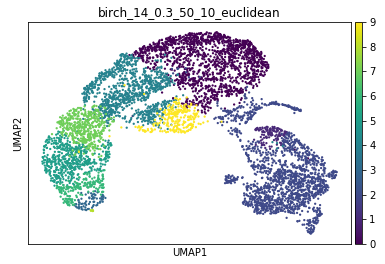
\includegraphics[width=0.22\textwidth]{birch-14-best.png}} 
    \subfigure{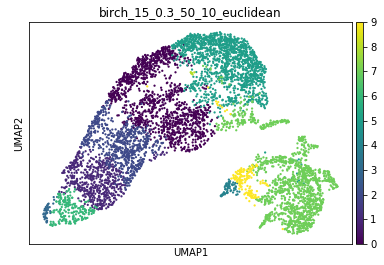
\includegraphics[width=0.22\textwidth]{birch-15-best.png}} 
    \subfigure{\includegraphics[width=0.22\textwidth]{birch-206-best.png}}
    \subfigure{\includegraphics[width=0.22\textwidth]{birch-207-best.png}}
    \caption{ Vizuelizacija rezultata dobijenih birhc algoritmom klasterovanja: }
    \label{fig:best_birch}
\end{figure}

\subsection{Zaključak}

Iako je korišćeno više metoda klasterovanja, na kraju su dobijeni veoma slični rezultati. 

\appendix{Vizualizacije}

\bibliographystyle{unsrt}  
\bibliography{references}
\end{document}
